\section{Stochastic approximation}

Let's take the online Q-learning algorithm developed in subsection \ref{ssec:model-free}.
The $\epsilon$-greedy strategy is used for this experiment.
Learning can be sped up using momentum acceleration, and Polyak averaging.

\subsubsection*{Momentum acceleration, per visit learning rate}

Let's modify the update rule for $\fn{Q}$ to the following:
\begin{equation}
	\fn{Q}_{n+1}(S, A) = (1 - \gamma_n)\,\fn{Q}_n(S, A) +
		\gamma_n\,\brc{R + \delta\,\underset{B\in\mathbb{A}}{\max}\fn{Q}(\widetilde{S}, B)} +
		\beta_n\,\left[\fn{Q}_n(S, A) - \fn{Q}_{n-1}(S, A)\right].
\end{equation}
$\beta_n$ is the coefficient of momentum acceleration. This method can increase convergence rate
and helps bypass local minima.

Moreover, set $\gamma_n = \frac{c_1}{\fn{n}(S, A)}$ and $\beta_n = \frac{c_2}{\fn{n}(S, A)}$.
$\fn{n}(S, A)$ denotes the number of visits to the state-action pair $(S, A)$, and $c_i$ are additional
coefficients.
This makes sure that rarely visited state-action pairs are updated with a sufficient learning rate.

\subsubsection*{Polyak averaging}

The purpose of Polyak averaging is to smooth out errors in $\fn{Q}_n$.
This is done by defining
\begin{equation}
	\widebar{\fn{Q}}_n = \frac{1}{\tau_n}\sum\limits_{t=n-\tau_n+1}^n\fn{Q}_t.
\end{equation}
Here, $\{\tau_n\}$ is the window width, such that $\tau_n\rightarrow\infty$ and $n-\tau_n\geq 0 $.
As an example, $\tau_n = \operatorname{ceil}(\log(n))$ was used.

The results are shown in figure \ref{fig:extension}.
Figure \ref{fig:IV-rew}. has been cropped so that it is more understandable.

\begin{figure}[H]
	\centering
	\begin{subfigure}{.46\textwidth}
		\centering
		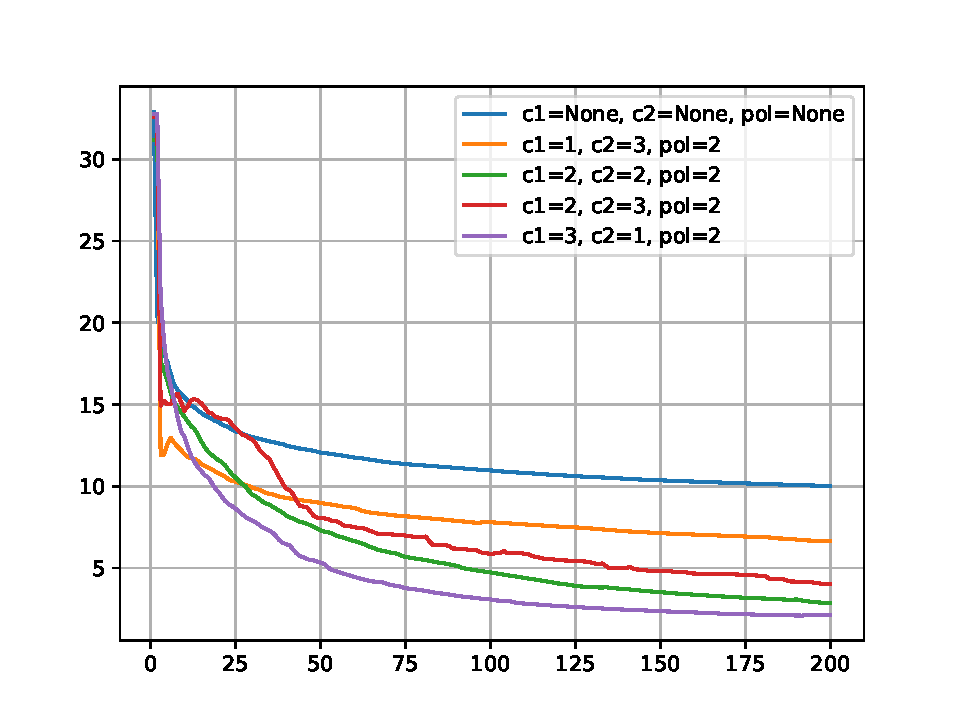
\includegraphics[width=\textwidth, trim={1cm, 0cm, 1cm, 1cm}, clip]{ex_IV_1_plots_dists}
		\caption{Distances from optimal value-function}
		\label{}
	\end{subfigure}\hfill
	\begin{subfigure}{.46\textwidth}
		\centering
		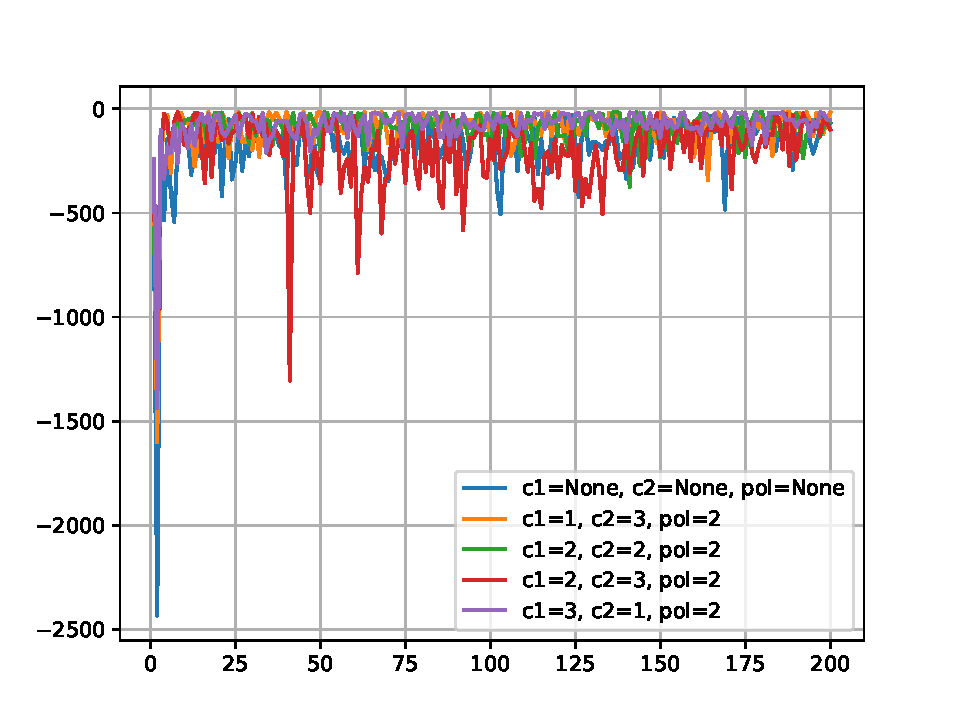
\includegraphics[width=\textwidth, trim={9mm, 0cm, 1cm, 1cm}, clip]{ex_IV_1_plots_rewards}
		\caption{Rewards at each iteration}
		\label{fig:IV-rew}
	\end{subfigure}
	\caption{Results of the extended Q-learning}
	\label{fig:extension}
\end{figure}
